% ============================================================
%  第 4 章  偏微分方程与特殊函数（扩展版）
% ============================================================

\chapter{偏微分方程与特殊函数}

\section{本章概览与学习路线}

牛顿第二定律 $\mathbf{F}=m\mathbf{a}$ 是常微分方程——描述的是单个质点的运动。但在连续介质（流体、弹性体、电磁场、量子波函数）中，物理量不仅是时间的函数，也是空间的函数。这就需要 \textbf{偏微分方程 (Partial Differential Equations, PDEs)}。

特殊函数不是数学家臆造的玩具，而是物理对称性在求解 PDE 过程中不可回避的产物——球对称 $\to$ 勒让德多项式，柱对称 $\to$ 贝塞尔函数，谐振子 $\to$ 埃尔米特多项式，氢原子 $\to$ 拉盖尔多项式。

\begin{center}
\fbox{\parbox{0.9\textwidth}{\centering
\textbf{核心逻辑链条：}\\
物理问题 $\to$ 三大 PDE 分类 $\to$ 对称性引导坐标系选择 $\to$ 分离变量 \\
$\to$ 本征值问题 $\to$ 特殊函数自然涌现 $\to$ SL 理论统一框架
}}
\end{center}

\subsection*{不同读者的学习路径}

\begin{itemize}
\item \textbf{物理专业学生：} 重点关注 \S4.2（三大 PDE 的物理含义）、\S4.3（分离变量法——量子力学和电磁学的基础）、\S4.4--\S4.5（勒让德和贝塞尔函数——原子物理和电磁散射的基础）。
\item \textbf{数学学生：} 重点关注 \S4.3（分离变量法的严格推导）、\S4.7（SL 理论的形式化框架）、\S4.8（球贝塞尔函数与散射理论）。
\item \textbf{工程学生：} 重点关注 \S4.2（三类 PDE 的判别与边界条件），\S4.3（分离变量法的算例），\S4.4--\S4.5（正交函数系的工程应用）。
\end{itemize}

\section{三大经典偏微分方程}
\label{sec:pde_types}

\subsection*{动机：物理学家只有这三类 PDE？}

几乎所有的物理定律都可以归入这三类：波动（信息传播）、扩散（信息模糊化）、稳态（场的静态平衡）。它们的区别不在于推导来源，而在于\textbf{特征线的结构}——也就是信息的传播方式。

\subsection{波动方程——双曲型}

\textbf{一维形式：}
\begin{equation}
\frac{\partial^2 u}{\partial t^2} = c^2 \frac{\partial^2 u}{\partial x^2},
\label{eq:wave1d}
\end{equation}
其中 $c$ 是波速。

\textbf{物理背景：} 弦的微小横振动中，张力 $T$ 和线密度 $\rho$ 决定了 $c = \sqrt{T/\rho}$。电磁波中 $c = 1/\sqrt{\mu_0\varepsilon_0}$。

\textbf{达朗贝尔解：} 对一维无界波动方程，通解为
\begin{equation}
u(x,t) = f(x-ct) + g(x+ct),
\end{equation}
即左右行波的叠加。

\textbf{达朗贝尔公式的推导：} 作变量代换 $\xi = x - ct$, $\eta = x + ct$，则波动方程化为 $\partial^2 u/\partial\xi\partial\eta = 0$。对 $\xi$ 积分得 $\partial u/\partial\eta = h(\eta)$，再对 $\eta$ 积分得 $u = \int h(\eta)\,\dd\eta + f(\xi) = f(\xi) + g(\eta)$。

\textbf{物理分类：}
\begin{itemize}
\item \textbf{双曲型}：信息以有限速度传播（特征线为 $x\pm ct = \text{常数}$）。
\item 初值问题的解由初始位移和初始速度唯一确定。
\item 能量守恒：机械能 $\int (\frac12 u_t^2 + \frac12 c^2 u_x^2)\,\dd x$ 不随时间变化。
\end{itemize}

\begin{insight}[双曲型方程的物理直觉]
双曲型 PDE 的核心特征是\textbf{有限传播速度}。这一点在狭义相对论中至关重要：如果信息可以超光速传播，因果律将被破坏。波动方程的特征线 $x \pm ct = \text{常数}$ 正是光锥在 $1+1$ 维时空中的投影。
\end{insight}

\subsection{热传导方程——抛物型}

\textbf{形式：}
\begin{equation}
\frac{\partial u}{\partial t} = \kappa \nabla^2 u.
\label{eq:heat}
\end{equation}

\textbf{物理背景：} $\kappa$ 是热扩散率。傅里叶热传导定律 $\mathbf{q} = -k\nabla T$（热流正比于温度梯度）结合能量守恒导出此方程。

\textbf{物理分类：}
\begin{itemize}
\item \textbf{抛物型}：信息以无限速度传播（解在 $t>0$ 后立即处处非零——但实际有意义的部分在扩散长度 $\sqrt{\kappa t}$ 内）。
\item 解是无限可微的（即使初始条件有间断，$t>0$ 后立刻光滑化）。
\item 熵增：温度梯度自发衰减，趋于均匀。
\end{itemize}

\begin{insight}[抛物型方程的物理直觉]
热传导方程展现了"时间之箭"：将 $t\to -t$ 替换，方程变为 $u_t = -\kappa u_{xx}$，这是向后热传导方程——物理上不可能，因为它需要从均匀温度场恢复初始的不均匀性。这正是\textbf{热力学第二定律}在 PDE 层面的体现。
\end{insight}

\subsection{泊松方程与拉普拉斯方程——椭圆型}

\textbf{形式：}
\begin{equation}
\nabla^2 u = -\frac{\rho}{\varepsilon_0}\quad\text{(泊松)},\qquad
\nabla^2 u = 0\quad\text{(拉普拉斯)}.
\label{eq:poisson_laplace}
\end{equation}

\textbf{物理分类：}
\begin{itemize}
\item \textbf{椭圆型}：稳态问题，不涉及时间演化。
\item 解由边界条件唯一确定（Dirichlet 或 Neumann 条件）。
\item 解具有"刚性"：最大值原理（调和函数的最大值必在边界上）。
\end{itemize}

\begin{theorem}[最大值原理]
若 $\nabla^2 u = 0$ 在有界区域 $\Omega$ 内成立且 $u\in C^2(\Omega)\cap C^0(\bar\Omega)$，则 $u$ 的最大值和最小值均在边界 $\partial\Omega$ 上达到。
\end{theorem}

最大值原理的物理意义：稳态热场中，内部任意点的温度不可能高于边界最高温度——否则热量会从内部流向边界，就不是稳态了。

% 三类 PDE 示意图
\begin{figure}[H]
\centering
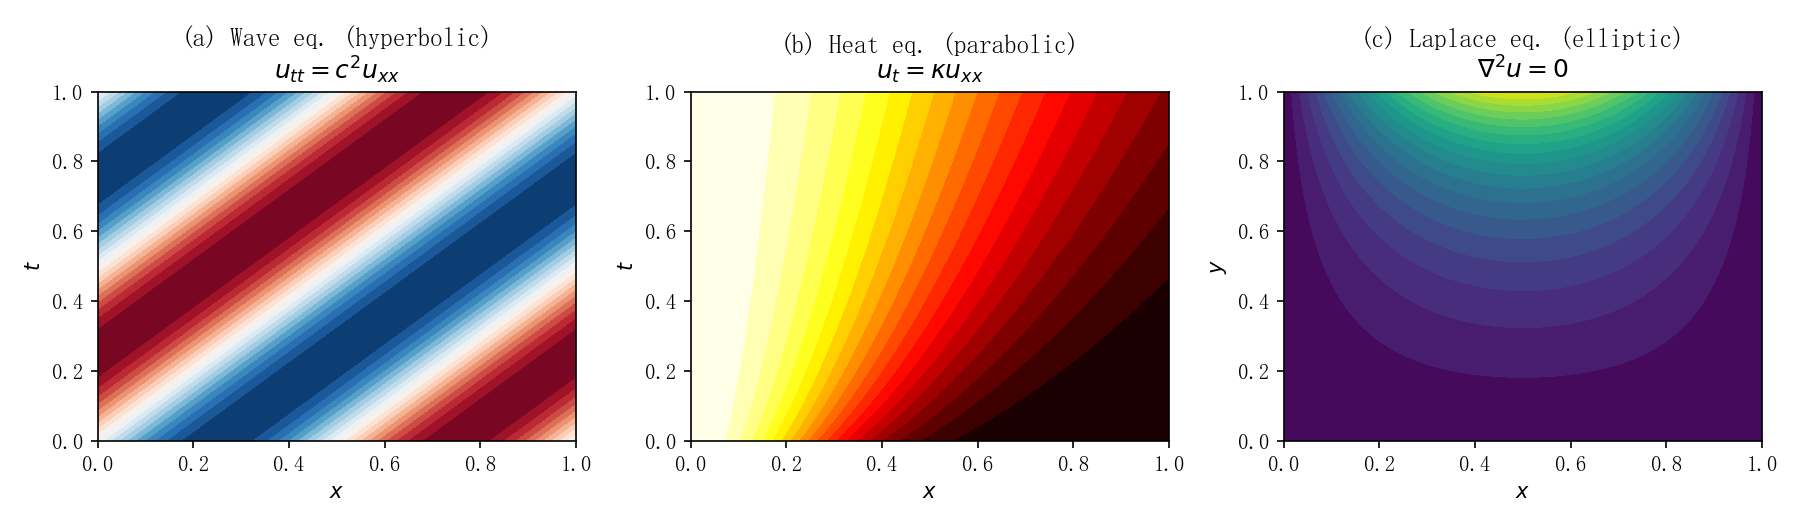
\includegraphics[width=0.85\textwidth]{figures/fig4_1_pde_types.png}
\caption{三类 PDE 的数值解示意图：(a) 波动方程（双曲型）——沿特征线传播的等相位线；(b) 热传导方程（抛物型）——温度扩散，前沿随 $\sqrt{t}$ 推进；(c) 拉普拉斯方程（椭圆型）——稳态分布，由边界条件唯一决定。}
\label{fig:pde_types}
\end{figure}

\subsection{PDE 的分类统一}

一般二阶线性 PDE 写为：
\begin{equation}
A\frac{\partial^2 u}{\partial x^2} + 2B\frac{\partial^2 u}{\partial x\partial y}
+ C\frac{\partial^2 u}{\partial y^2} + \text{(低阶项)} = 0.
\end{equation}

分类由判别式 $\Delta = B^2 - AC$ 决定：
\begin{itemize}
\item $\Delta > 0$：\textbf{双曲型}（波动方程），两条实特征线。
\item $\Delta = 0$：\textbf{抛物型}（热传导方程），一条实特征线。
\item $\Delta < 0$：\textbf{椭圆型}（拉普拉斯方程），无实特征线。
\end{itemize}

这个分类名称来源于二次型 $A\xi^2 + 2B\xi\eta + C\eta^2$ 的几何类型，与圆锥曲线的分类完全一致。

\begin{example}[PDE 分类练习]
判断下列方程的类型：

\textbf{(1)} $u_{xx} + 2u_{xy} + u_{yy} = 0$：$A=1,B=1,C=1$，$\Delta = 1-1 = 0$，抛物型。

\textbf{(2)} $u_{xx} - 3u_{yy} = 0$：$A=1,B=0,C=-3$，$\Delta = 0-(-3) = 3 > 0$，双曲型。

\textbf{(3)} $u_{xx} + u_{yy} + u_{zz} = 0$：三维拉普拉斯方程，椭圆型。

\textbf{(4)} $u_t = u_{xx} + u_{yy}$：二维热传导方程，抛物型（对 $t$ 一阶、对 $x,y$ 二阶）。
\end{example}

\section{分离变量法}
\label{sec:separation}

\subsection*{动机：如何把 PDE 拆成 ODE？}

分离变量法的核心想法很直接：假设 $u(x,t)=X(x)T(t)$，代入 PDE 后，等号两边分别是 $x$ 的函数和 $t$ 的函数。要使它们对所有 $x,t$ 都相等，只有一种可能：两边都等于同一个常数。这个常数就是\textbf{分离常数}，它将在后续步骤中引出本征值问题。

\subsection{一般步骤}

分离变量法的标准流程：

\begin{enumerate}
\item \textbf{假设分离变量形式} $u(x,t) = X(x)T(t)$（或 $u(x,y) = X(x)Y(y)$ 等）。
\item \textbf{代入 PDE 并分离}，得到两个（或更多）常微分方程和一个分离常数。
\item \textbf{求解本征值问题}——空间 ODE + 齐次边界条件给出本征值和本征函数。
\item \textbf{求解时间 ODE}——每个本征值对应一个时间演化模式。
\item \textbf{叠加所有模式}，由非齐次初始条件通过正交性确定展开系数。
\end{enumerate}

\subsection{一维波动方程（两端固定弦）}

\begin{align}
\frac{\partial^2 u}{\partial t^2} &= c^2 \frac{\partial^2 u}{\partial x^2},\quad
0<x<L,\\
u(0,t) &= u(L,t) = 0,\\
u(x,0) &= f(x),\quad u_t(x,0) = g(x).
\end{align}

\textbf{第一步：设 $u(x,t) = X(x)T(t)$，代入得}
\begin{equation}
X T'' = c^2 X'' T \quad\Longrightarrow\quad
\frac{T''}{c^2 T} = \frac{X''}{X} = -\lambda.
\end{equation}

\textbf{第二步：求解空间 ODE（本征值问题）}
\begin{equation}
X'' + \lambda X = 0,\quad X(0)=X(L)=0.
\end{equation}

本征值和本征函数：
\begin{equation}
\lambda_n = \left(\frac{n\pi}{L}\right)^2,\quad
X_n(x) = \sin\frac{n\pi x}{L},\quad n=1,2,3,\dots
\label{eq:wave_eigen}
\end{equation}

\textbf{第三步：求解时间 ODE}
\begin{equation}
T''_n + c^2\lambda_n T_n = 0 \quad\Longrightarrow\quad
T_n(t) = A_n\cos(\omega_n t) + B_n\sin(\omega_n t),
\end{equation}
其中 $\omega_n = n\pi c/L$ 是第 $n$ 阶固有频率。

\textbf{第四步：叠加并利用初始条件确定系数}
\begin{align}
u(x,t) &= \sum_{n=1}^{\infty} \sin\frac{n\pi x}{L}
\left[A_n\cos(\omega_n t) + B_n\sin(\omega_n t)\right],\\
A_n &= \frac{2}{L}\int_0^L f(x)\sin\frac{n\pi x}{L}\,\dd x,\\
B_n &= \frac{2}{n\pi c}\int_0^L g(x)\sin\frac{n\pi x}{L}\,\dd x.
\end{align}

\begin{insight}
本征函数 $\sin(n\pi x/L)$ 正是傅里叶正弦级数的基函数。分离变量法在此处自然引出傅里叶级数——不是我们"选择"了正弦函数，而是两端固定的边界条件\textbf{强迫}本征函数必须是正弦函数。这就是物理对称性决定数学形式的绝佳例证。
\end{insight}

\subsection{一维热传导方程——完整算例}

\begin{example}[两端固定温度的杆]
一根长度为 $L$ 的均匀细杆，初始温度分布为 $u(x,0)=T_0\sin(\pi x/L)$，两端温度保持 $u(0,t)=u(L,t)=0$。求温度分布 $u(x,t)$。

\textbf{步骤 1：分离变量。}
设 $u(x,t)=X(x)T(t)$，代入 $u_t = \kappa u_{xx}$：
\begin{equation}
\frac{T'}{\kappa T} = \frac{X''}{X} = -\lambda.
\end{equation}

\textbf{步骤 2：空间 ODE。}
$X'' + \lambda X = 0$，$X(0)=X(L)=0$。
与波动方程相同：$\lambda_n = (n\pi/L)^2$，$X_n(x)=\sin(n\pi x/L)$。

\textbf{步骤 3：时间 ODE。}
$T'_n = -\kappa\lambda_n T_n$，解得 $T_n(t) = C_n e^{-\kappa (n\pi/L)^2 t}$。

\textbf{步骤 4：一般解。}
\begin{equation}
u(x,t) = \sum_{n=1}^{\infty} C_n \sin\frac{n\pi x}{L} e^{-\kappa (n\pi/L)^2 t}.
\end{equation}

\textbf{步骤 5：代入初始条件。}
\begin{equation}
u(x,0) = \sum_{n=1}^{\infty} C_n \sin\frac{n\pi x}{L} = T_0\sin\frac{\pi x}{L}.
\end{equation}
由正弦级数的正交性：$C_1 = T_0$，$C_n=0$（$n\geq2$）。

\textbf{步骤 6：最终解。}
\begin{equation}
\boxed{\;u(x,t) = T_0\sin\frac{\pi x}{L}\, e^{-\kappa(\pi/L)^2 t}\;}.
\end{equation}

\textbf{物理解读：} 温度呈正弦分布，整体指数衰减，衰减时间常数 $\tau = (L/\pi)^2/\kappa$。杆越长，衰减越慢。
\end{example}

\subsection{二维拉普拉斯方程（矩形区域）}

\begin{equation}
\frac{\partial^2 u}{\partial x^2} + \frac{\partial^2 u}{\partial y^2} = 0,\quad
0<x<a,\;0<y<b.
\end{equation}

边界条件：$u(0,y)=u(a,y)=0$，$u(x,0)=0$，$u(x,b)=f(x)$。

分离变量 $u(x,y)=X(x)Y(y)$：
\begin{equation}
\frac{X''}{X} = -\frac{Y''}{Y} = -k^2.
\end{equation}

$X$ 方程的解：$X_n(x) = \sin\frac{n\pi x}{a}$（$n=1,2,\dots$）。
$Y$ 方程：$Y_n'' = k_n^2 Y_n$，$k_n = n\pi/a$。

满足 $Y_n(0)=0$ 的解为 $Y_n(y) = \sinh(k_n y)$。最终解：
\begin{equation}
u(x,y) = \sum_{n=1}^{\infty} c_n \sin\frac{n\pi x}{a}\,
\sinh\frac{n\pi y}{a},
\end{equation}
其中 $c_n$ 由 $u(x,b)=f(x)$ 确定：
\begin{equation}
c_n = \frac{2}{a\sinh(k_n b)}\int_0^a f(x)\sin\frac{n\pi x}{a}\,\dd x.
\end{equation}

\subsection{球对称：三维拉普拉斯方程}

在球坐标中，拉普拉斯方程为：
\begin{equation}
\frac{1}{r^2}\frac{\partial}{\partial r}\left(r^2\frac{\partial u}{\partial r}\right)
+ \frac{1}{r^2\sin\theta}\frac{\partial}{\partial\theta}\left(\sin\theta\frac{\partial u}{\partial\theta}\right)
+ \frac{1}{r^2\sin^2\theta}\frac{\partial^2 u}{\partial\phi^2} = 0.
\end{equation}

分离变量 $u(r,\theta,\phi) = R(r)\Theta(\theta)\Phi(\phi)$ 得到三个 ODE：
\begin{align}
\frac{1}{\Phi}\frac{\dd^2\Phi}{\dd\phi^2} &= -m^2,\\
\frac{1}{\sin\theta}\frac{\dd}{\dd\theta}\left(\sin\theta\frac{\dd\Theta}{\dd\theta}\right)
+ \left[l(l+1) - \frac{m^2}{\sin^2\theta}\right]\Theta &= 0,\\
\frac{1}{r^2}\frac{\dd}{\dd r}\left(r^2\frac{\dd R}{\dd r}\right)
- \frac{l(l+1)}{r^2}R &= 0.
\end{align}

角向方程的解是\textbf{球谐函数} $Y_{lm}(\theta,\phi)$，径向方程的解是 $r^l$ 和 $r^{-(l+1)}$。这正是静电场中多极展开的基础。

\section{勒让德多项式}
\label{sec:legendre}

\subsection*{动机：球对称问题为什么必然出现勒让德多项式？}

在球坐标中分离变量后，$\theta$ 方向的方程（经过变换 $x=\cos\theta$）就是勒让德方程。要求解在 $\theta=0,\pi$（南北极）处有限，$l$ 必须为整数——这就是角动量量子化的数学起源！勒让德多项式不是一个"可以选"的基函数，而是物理约束（有界性）迫使的唯一选择。

\subsection{勒让德方程}

$\theta$ 方程在令 $x = \cos\theta$ 后化为\textbf{勒让德方程} ($m=0$ 时)：
\begin{equation}
(1-x^2)\frac{\dd^2 P}{\dd x^2} - 2x\frac{\dd P}{\dd x}
+ l(l+1)P = 0,\qquad x\in[-1,1].
\label{eq:legendre_ode}
\end{equation}

该方程在 $x=\pm1$ 处具有正则奇点。要求解在 $x=\pm1$ 处有界——即物理上在球轴的南北极温度/势有限——这迫使 $l$ 为非负整数。

\subsection{勒让德多项式}

$l$ 为整数时，勒让德方程的多项式解称为\textbf{勒让德多项式}：
\begin{align}
P_0(x) &= 1,\\
P_1(x) &= x,\\
P_2(x) &= \frac{1}{2}(3x^2-1),\\
P_3(x) &= \frac{1}{2}(5x^3-3x),\\
P_4(x) &= \frac{1}{8}(35x^4-30x^2+3).
\end{align}

\textbf{罗德里格斯公式：}
\begin{equation}
P_l(x) = \frac{1}{2^l l!}\frac{\dd^l}{\dd x^l}(x^2-1)^l.
\label{eq:rodrigues}
\end{equation}

\textbf{递推关系：}
\begin{equation}
(l+1)P_{l+1}(x) = (2l+1)xP_l(x) - lP_{l-1}(x).
\end{equation}
由 $P_0(x)=1$, $P_1(x)=x$ 和递推关系可以生成所有高阶勒让德多项式。

\textbf{正交性：}
\begin{equation}
\int_{-1}^{1} P_l(x)P_{l'}(x)\,\dd x = \frac{2}{2l+1}\delta_{ll'}.
\label{eq:legendre_ortho}
\end{equation}

\textbf{完备性：} $[-1,1]$ 上的任意良函数可以展开为勒让德级数：
\begin{equation}
f(x) = \sum_{l=0}^{\infty} A_l P_l(x),\quad
A_l = \frac{2l+1}{2}\int_{-1}^{1} f(x)P_l(x)\,\dd x.
\end{equation}

% 勒让德多项式图
\begin{figure}[H]
\centering
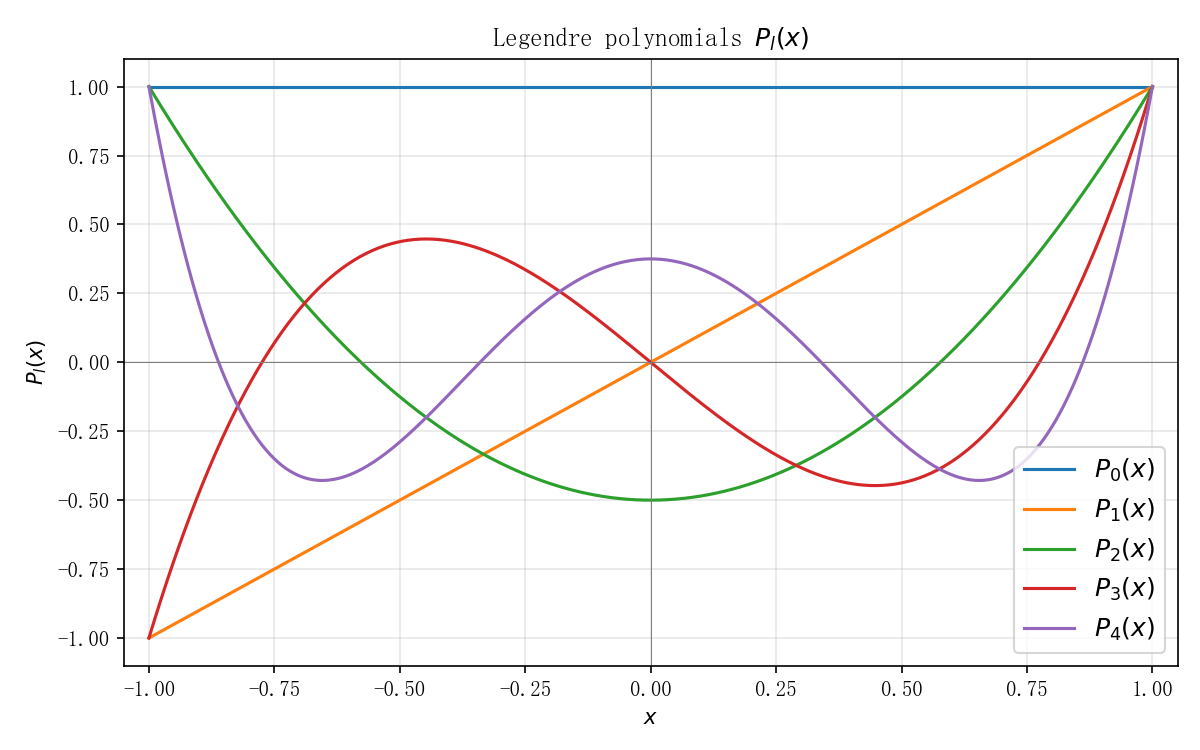
\includegraphics[width=0.6\textwidth]{figures/fig4_2_legendre.png}
\caption{前 5 阶勒让德多项式 $P_l(x)$。注意：$P_l(1)=1$ 对所有 $l$ 成立；$P_l$ 在 $(-1,1)$ 内有 $l$ 个零点。}
\label{fig:legendre}
\end{figure}

\subsection{物理应用：静电场的多极展开}

在远离电荷分布的区域，电势可以按勒让德多项式展开：
\begin{equation}
\phi(r,\theta) = \frac{1}{4\pi\varepsilon_0}\sum_{l=0}^{\infty}
\frac{1}{r^{l+1}}P_l(\cos\theta)\int r'^l P_l(\cos\theta')\rho(\mathbf{r}')\,\dd V'.
\end{equation}

\textbf{前三项：}
\begin{itemize}
\item $l=0$：单极项 $\phi_0 = \dfrac{Q}{4\pi\varepsilon_0 r}$，$Q$ 为总电荷。
\item $l=1$：偶极项 $\phi_1 = \dfrac{\mathbf{p}\cdot\mathbf{r}}{4\pi\varepsilon_0 r^3}$，$\mathbf{p} = \int \mathbf{r}'\rho\,\dd V'$ 为电偶极矩。
\item $l=2$：四极项 $\phi_2 = \dfrac{1}{4\pi\varepsilon_0}\dfrac{1}{2r^5}\sum_{ij} Q_{ij}x_i x_j$，$Q_{ij}$ 为四极矩张量。
\end{itemize}

\begin{insight}
多极展开的物理意义：远场电势由总电荷（单极）主导，当总电荷为零时由偶极主导，以此类推。这如同傅里叶级数在空间角域中的对应——将电荷分布的角向结构分解为不同"空间频率"的成分。实验物理中，通过测量远场多极矩可以反推源分布的对称性——这正是原子核形状和分子结构的诊断工具。
\end{insight}

\subsection{连带勒让德函数与球谐函数}

对于 $m\neq0$ 的情况，方程的解是\textbf{连带勒让德函数}：
\begin{equation}
P_l^m(x) = (1-x^2)^{m/2}\frac{\dd^m}{\dd x^m}P_l(x),\qquad -l\leq m\leq l.
\label{eq:associated_legendre}
\end{equation}

球谐函数为：
\begin{equation}
Y_{lm}(\theta,\phi) = (-1)^m\sqrt{\frac{2l+1}{4\pi}\frac{(l-m)!}{(l+m)!}}
P_l^m(\cos\theta)e^{\mathrm{i}m\phi}.
\label{eq:spherical_harmonic}
\end{equation}

\textbf{正交归一：}
\begin{equation}
\int_0^{2\pi}\int_0^{\pi} Y_{lm}^*(\theta,\phi)Y_{l'm'}(\theta,\phi)\,
\sin\theta\,\dd\theta\,\dd\phi = \delta_{ll'}\delta_{mm'}.
\end{equation}

球谐函数是 $\hat{L}^2$ 和 $\hat{L}_z$ 的共同本征函数，也是 $L^2(S^2)$（二维球面上的平方可积函数空间）的完备正交基。任何球面上的函数（如地磁场分布、CMB 温度图）都可以展开为球谐级数。

% 球谐函数图
\begin{figure}[H]
\centering
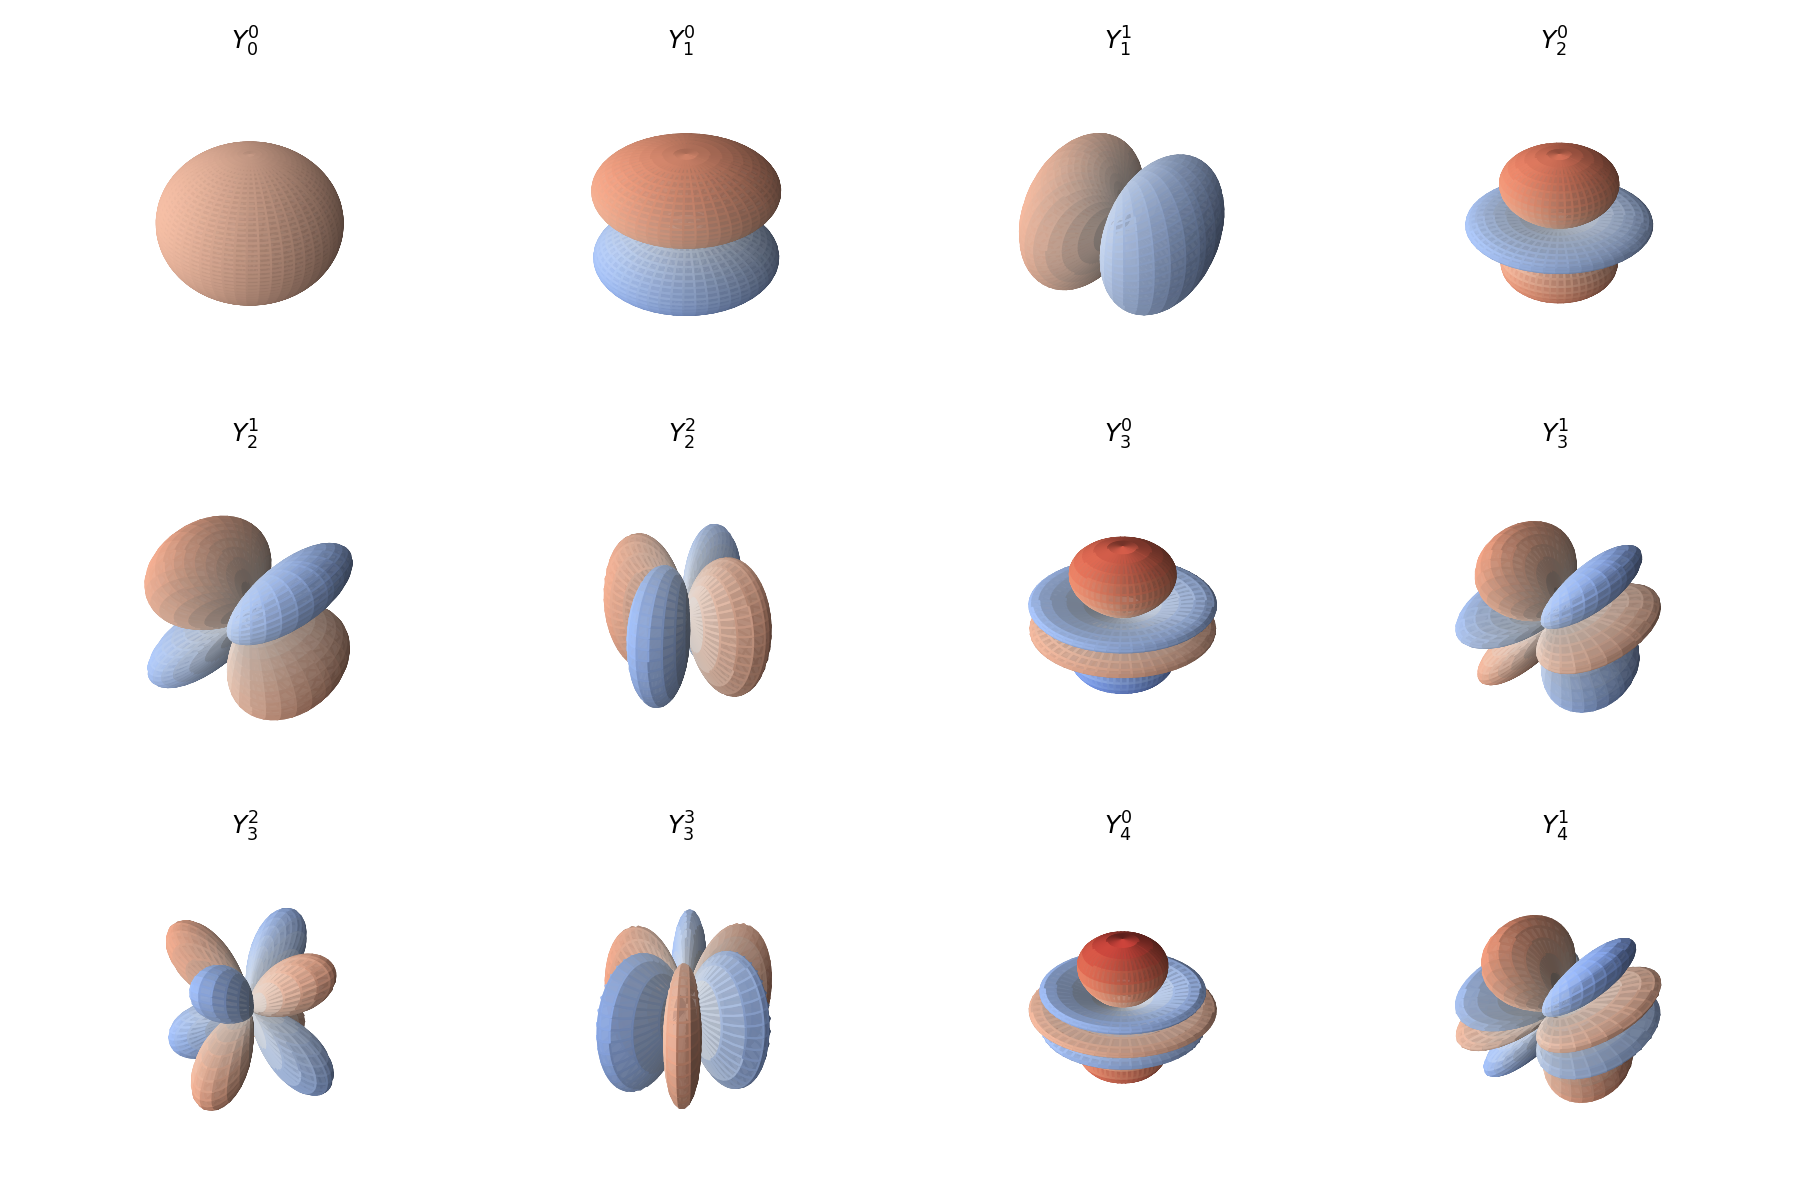
\includegraphics[width=0.85\textwidth]{figures/fig4_5_spherical_harmonics.png}
\caption{球谐函数 $Y_l^m(\theta,\phi)$ 的 3D 可视化。颜色表示实部的正负，径向距离表示 $|Y_l^m|$ 的大小。$l$ 增加意味着角向振荡加快。}
\label{fig:spherical_harmonics}
\end{figure}

\section{贝塞尔函数}
\label{sec:bessel}

\subsection*{动机：柱对称问题为什么产生贝塞尔函数？}

与球对称类似，在柱坐标或极坐标中分离变量后，径向方程变为贝塞尔方程。贝塞尔函数 $J_0(x)$ 描述了圆膜振动、圆柱波导中的电磁场分布、以及热传导中的径向温度分布。它的关键特征是：在 $x=0$ 处有限，在大 $x$ 处像 $\cos(x)/\sqrt{x}$ 衰减——这正是"柱面波"的几何稀释效应。

\subsection{贝塞尔方程}

在柱坐标或极坐标中对拉普拉斯方程、波动方程或热传导方程分离变量时，径向方程通常化为\textbf{贝塞尔方程}：
\begin{equation}
x^2\frac{\dd^2 y}{\dd x^2} + x\frac{\dd y}{\dd x} + (x^2 - \nu^2)y = 0.
\label{eq:bessel_ode}
\end{equation}

其中 $\nu$ 是阶数，由分离变量常数 $m$ 决定。在柱对称问题中，$\nu = m$（整数）。

\subsection{第一类贝塞尔函数}

贝塞尔方程的两个线性无关解是 $J_\nu(x)$ 和 $Y_\nu(x)$（或 $N_\nu(x)$），分别称为\textbf{第一类和第二类贝塞尔函数}。

$J_\nu(x)$ 的级数表示：
\begin{equation}
J_\nu(x) = \sum_{k=0}^{\infty}
\frac{(-1)^k}{k!\,\Gamma(\nu+k+1)}\left(\frac{x}{2}\right)^{\nu+2k}.
\label{eq:bessel_series}
\end{equation}

\textbf{渐近行为：}
\begin{align}
J_\nu(x) &\sim \frac{1}{\Gamma(\nu+1)}\left(\frac{x}{2}\right)^\nu,\quad x\to 0,\\
J_\nu(x) &\sim \sqrt{\frac{2}{\pi x}}\cos\left(x - \frac{\nu\pi}{2} - \frac{\pi}{4}\right),\quad x\to\infty.
\label{eq:bessel_asym}
\end{align}

\textbf{递推关系：}
\begin{align}
J_{\nu-1}(x) + J_{\nu+1}(x) &= \frac{2\nu}{x}J_\nu(x),\\
J_{\nu-1}(x) - J_{\nu+1}(x) &= 2J'_\nu(x).
\end{align}

\begin{insight}
$J_\nu(x)$ 在 $x\to\infty$ 时像衰减的正弦波，这正是"径向波动"的特征：
\begin{itemize}
\item $1/\sqrt{x}$ 衰减：二维或三维波在扩展中的能量稀释。
\item 余弦相位：波从原点径向向外传播。
\end{itemize}
对比之下，勒让德多项式在 $x\in[-1,1]$ 上振荡但幅度恒定——因为它是角向函数，不存在几何扩散效应。
\end{insight}

% 贝塞尔函数图
\begin{figure}[H]
\centering
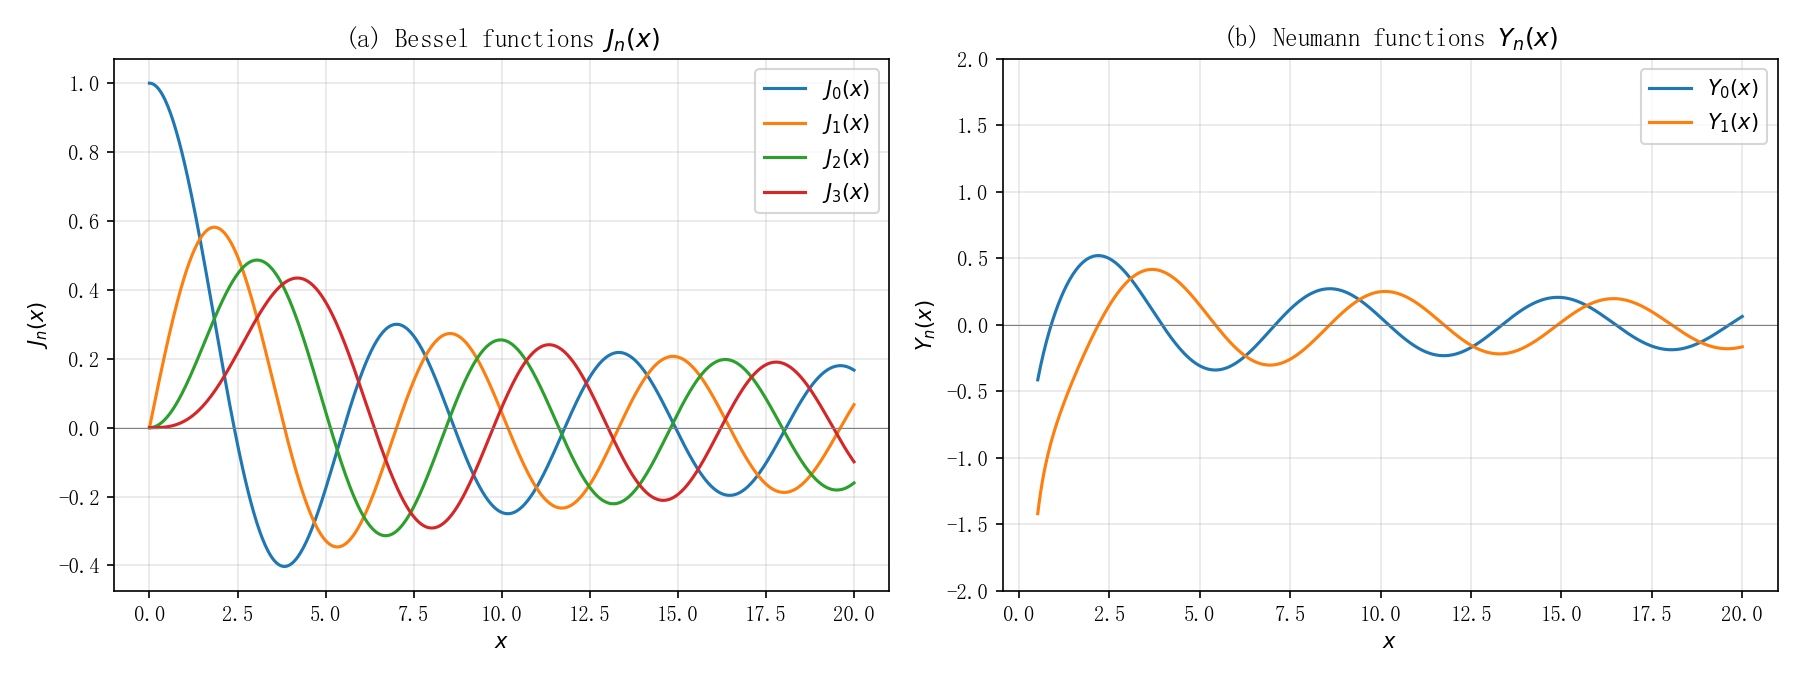
\includegraphics[width=0.85\textwidth]{figures/fig4_3_bessel.png}
\caption{(a) 第一类贝塞尔函数 $J_n(x)$（$n=0,1,2,3$）。(b) 第二类（诺依曼函数）$Y_n(x)$。注意 $Y_n(0)\to -\infty$，因此在涉及原点的物理问题中通常只保留 $J_n$。}
\label{fig:bessel}
\end{figure}

\subsection{贝塞尔函数的正交性}

对于固定 $\nu$，设 $j_{\nu,n}$ 为 $J_\nu(x)=0$ 的第 $n$ 个正根。则 $\{J_\nu(j_{\nu,n}\,r/R)\}$ 在区间 $[0,R]$ 上关于权重 $r$ 正交：
\begin{equation}
\int_0^R J_\nu\!\left(\frac{j_{\nu,m}r}{R}\right)
J_\nu\!\left(\frac{j_{\nu,n}r}{R}\right) r\,\dd r
= \frac{R^2}{2}[J_{\nu+1}(j_{\nu,n})]^2\delta_{mn}.
\label{eq:bessel_ortho}
\end{equation}

\subsection{物理应用：圆膜振动——完整算例}

\begin{example}[圆形鼓膜的振动模式]
\textbf{问题：} 半径为 $a$ 的圆形鼓膜，边界固定 $u(a,\phi)=0$。求振动模式（本征频率和本征函数）。

\textbf{步骤 1：建立极坐标波动方程。}
\begin{equation}
\frac{\partial^2 u}{\partial t^2} = c^2\left[
\frac{1}{r}\frac{\partial}{\partial r}\left(r\frac{\partial u}{\partial r}\right)
+ \frac{1}{r^2}\frac{\partial^2 u}{\partial\phi^2}
\right].
\end{equation}

\textbf{步骤 2：分离变量。}
$u(r,\phi,t)=R(r)\Phi(\phi)T(t)$。
\begin{align}
\frac{T''}{c^2 T} &= -k^2,\\
\frac{\Phi''}{\Phi} &= -m^2,\\
r^2 R'' + rR' + (k^2 r^2 - m^2)R &= 0.
\end{align}

\textbf{步骤 3：时间解。}
$T'' + k^2 c^2 T = 0 \Rightarrow T(t) = A\cos(\omega t) + B\sin(\omega t)$，其中 $\omega = kc$。

\textbf{步骤 4：角向解。}
$\Phi(\phi) = e^{\mathrm{i}m\phi}$，$m=0,1,2,\dots$（周期性要求 $m$ 为整数）。

\textbf{步骤 5：径向解——贝塞尔函数。}
径向方程是 $\nu=m$ 的贝塞尔方程。解为 $R(r) = J_m(kr)$（要求 $r=0$ 处有限，排除 $Y_m$）。

\textbf{步骤 6：边界条件确定 $k$。}
$u(a,\phi,t)=0 \Rightarrow R(a)=0 \Rightarrow J_m(ka)=0$。
令 $j_{m,n}$ 为 $J_m$ 的第 $n$ 个正零点，则 $k = j_{m,n}/a$，$n=1,2,3,\dots$。

\textbf{步骤 7：本征频率。}
\begin{equation}
\boxed{\;\omega_{mn} = c\,\frac{j_{m,n}}{a},\qquad
f_{mn} = \frac{c\,j_{m,n}}{2\pi a}\;}.
\end{equation}

\textbf{步骤 8：物理解读。}
基频：$(m,n)=(0,1)$ 对应 $j_{0,1}\approx 2.405$，$f_{01}=0.383c/a$——全膜同向振动。
一阶泛音：$(m,n)=(1,1)$ 对应 $j_{1,1}\approx 3.832$，有一条直径节线。
这些频率并非整数倍关系——鼓的声音"不和谐"的数学根源正在于此。
\end{example}

% 圆膜振动模式
\begin{figure}[H]
\centering
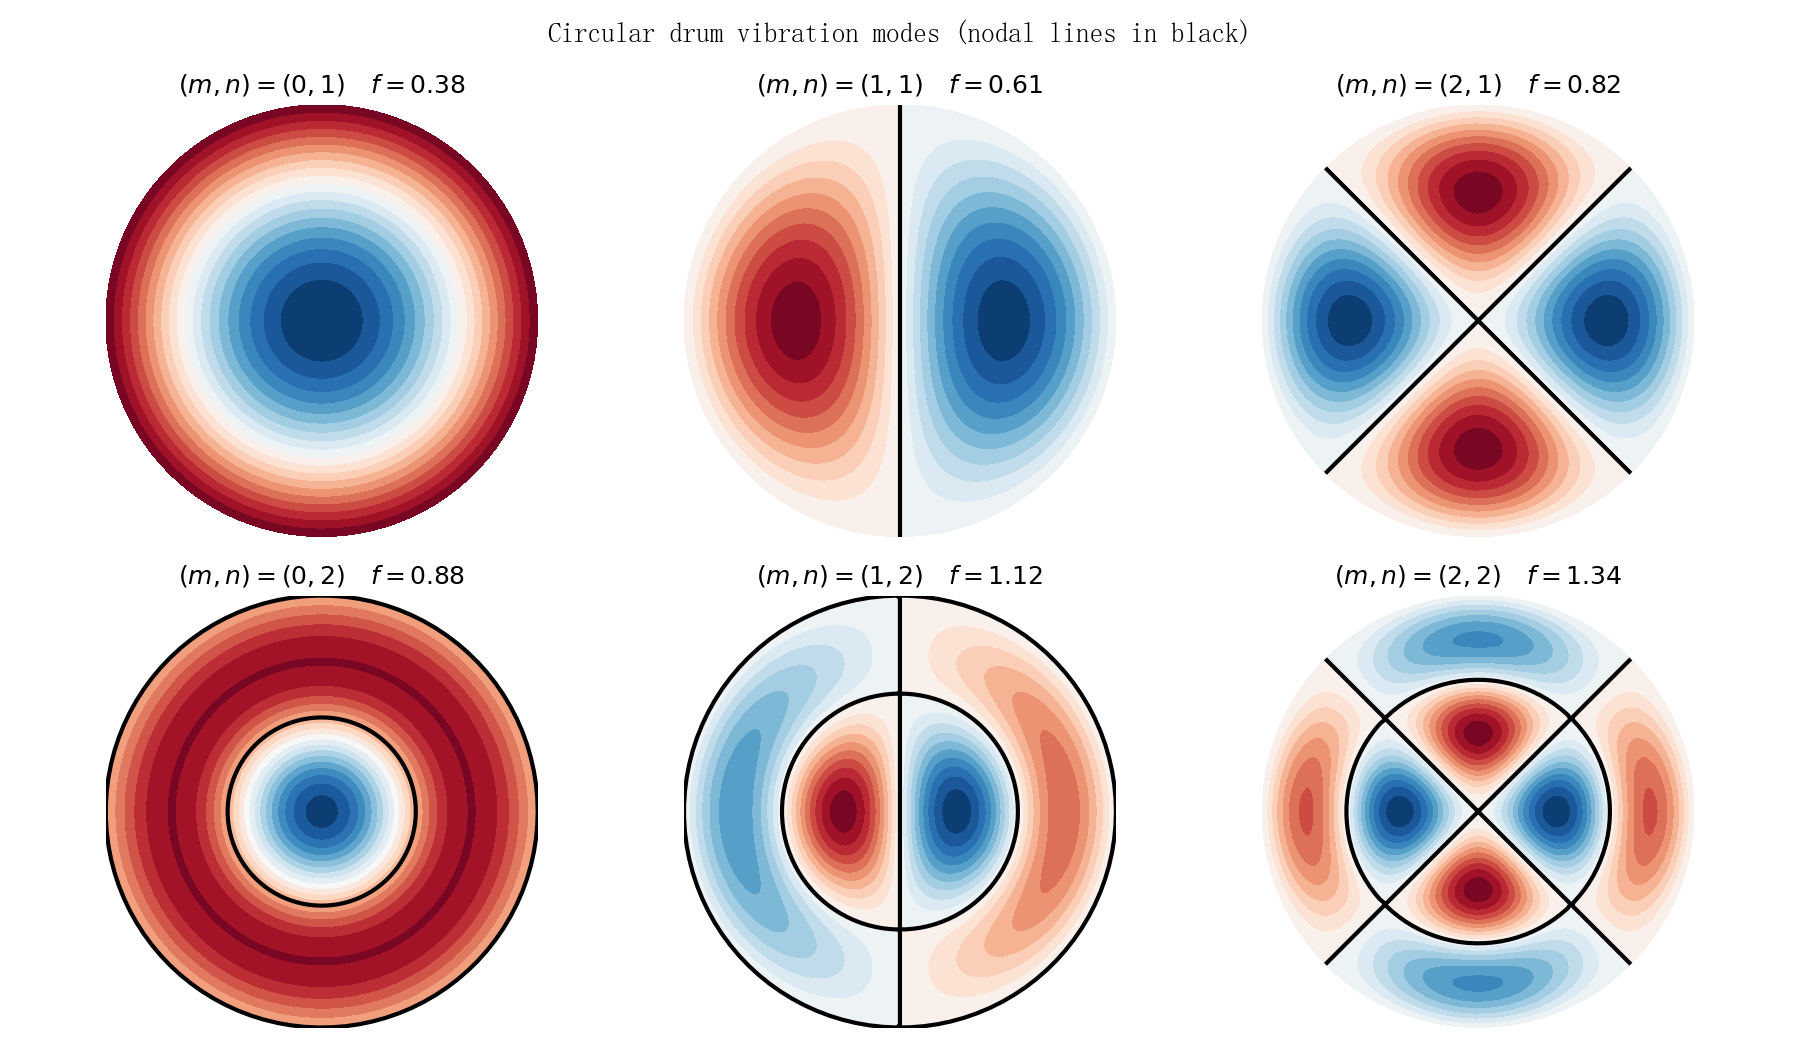
\includegraphics[width=0.85\textwidth]{figures/fig4_4_drum_modes.png}
\caption{圆膜的振动模式。颜色表位移，黑线为节线（位移恒为零的线）。$(m,n)$ 中 $m$ 为直径节线数，$n$ 为环向节线数。频率 $f$ 增加随 $m,n$ 增大而增大。}
\label{fig:drum_modes}
\end{figure}

\section{埃尔米特多项式与量子谐振子}
\label{sec:hermite}

\subsection*{动机：为什么量子谐振子产生离散能级？}

量子谐振子 $V(x) = \frac12 m\omega^2 x^2$ 的定态薛定谔方程在分离变量后，自然引出埃尔米特方程。其解——埃尔米特多项式——的正交性和递推关系直接给出了能级的量子化结构和升降算符。

\subsection{量子谐振子的定态薛定谔方程}

一维谐振子的定态薛定谔方程：
\begin{equation}
-\frac{\hbar^2}{2m}\frac{\dd^2\psi}{\dd x^2} + \frac12 m\omega^2 x^2\psi = E\psi.
\end{equation}

引入无量纲变量 $\xi = \sqrt{m\omega/\hbar}\,x$，方程化为：
\begin{equation}
\frac{\dd^2\psi}{\dd\xi^2} + (\epsilon - \xi^2)\psi = 0,\quad \epsilon = \frac{2E}{\hbar\omega}.
\label{eq:hermite_ode_raw}
\end{equation}

\subsection{埃尔米特方程与多项式}

设 $\psi(\xi) = H(\xi)e^{-\xi^2/2}$，代入后得到\textbf{埃尔米特方程}：
\begin{equation}
\frac{\dd^2 H}{\dd\xi^2} - 2\xi\frac{\dd H}{\dd\xi} + (\epsilon - 1)H = 0.
\label{eq:hermite_ode}
\end{equation}

要求波函数在无穷远处有限，迫使 $\epsilon - 1 = 2n$，即 $n=0,1,2,\dots$。此时方程的多项式解为\textbf{埃尔米特多项式}：

\begin{align}
H_0(\xi) &= 1,\\
H_1(\xi) &= 2\xi,\\
H_2(\xi) &= 4\xi^2 - 2,\\
H_3(\xi) &= 8\xi^3 - 12\xi,\\
H_4(\xi) &= 16\xi^4 - 48\xi^2 + 12.
\end{align}

\textbf{罗德里格斯公式：}
\begin{equation}
H_n(\xi) = (-1)^n e^{\xi^2}\frac{\dd^n}{\dd\xi^n}e^{-\xi^2}.
\label{eq:hermite_rodrigues}
\end{equation}

\textbf{正交性：}
\begin{equation}
\int_{-\infty}^{\infty} H_n(\xi)H_m(\xi)e^{-\xi^2}\,\dd\xi
= 2^n n!\sqrt{\pi}\,\delta_{nm}.
\label{eq:hermite_ortho}
\end{equation}

\textbf{递推关系：}
\begin{equation}
H_{n+1}(\xi) = 2\xi H_n(\xi) - 2n H_{n-1}(\xi),\qquad
H'_n(\xi) = 2n H_{n-1}(\xi).
\end{equation}

\subsection{量子谐振子的本征解}

\textbf{能级：}
\begin{equation}
E_n = \left(n + \frac12\right)\hbar\omega,\qquad n=0,1,2,\dots
\end{equation}

\textbf{本征函数：}
\begin{equation}
\psi_n(x) = \frac{1}{\sqrt{2^n n!}}\left(\frac{m\omega}{\pi\hbar}\right)^{1/4}
H_n\!\left(\sqrt{\frac{m\omega}{\hbar}}\,x\right) e^{-m\omega x^2/(2\hbar)}.
\label{eq:harmonic_oscillator_wf}
\end{equation}

\begin{insight}
埃尔米特多项式的递推关系 $H_{n+1} = 2\xi H_n - 2n H_{n-1}$ 在量子力学中有深刻的物理对应——它正是\textbf{升降算符} $\hat{a}^\dagger$ 和 $\hat{a}$ 作用的数学表现。这种代数方法（ ladder operator）远比直接求解微分方程优雅，也是量子场论中产生/湮灭算符的原型。
\end{insight}

\section{施图姆-刘维尔理论}
\label{sec:sturm_liouville}

\subsection*{动机：为什么所有特殊函数都有相同的正交性？}

勒让德多项式的正交关系 $\int_{-1}^1 P_l P_{l'} = 2/(2l+1)\delta_{ll'}$ 和贝塞尔函数的正交关系 $\int_0^R J_m(jr/R)J_m(j'r/R) r\,dr \propto \delta_{jj'}$，虽然看起来不同，但本质上来自同一个原因：它们都是\textbf{自伴算符}的本征函数。这就是施图姆-刘维尔理论的意义——它统一了所有正交函数系。

\subsection{SL 问题的标准形式}

\begin{equation}
-\frac{\dd}{\dd x}\left[p(x)\frac{\dd y}{\dd x}\right] + q(x)y
= \lambda w(x)y,\qquad a<x<b,
\label{eq:sl_form}
\end{equation}
附加适当的边界条件。

\textbf{SL 理论的核心结论：}
\begin{enumerate}
\item 本征值 $\lambda_n$ 是实数，且构成递增序列 $\lambda_1<\lambda_2<\cdots\to\infty$。
\item 本征函数 $y_n(x)$ 关于权函数 $w(x)$ 正交：
\begin{equation}
\int_a^b y_n(x) y_m(x) w(x)\,\dd x = 0,\quad n\neq m.
\end{equation}
\item 本征函数构成完备集——任意满足边界条件的函数可按 $\{y_n\}$ 展开。
\end{enumerate}

\subsection{SL 问题的物理统一性}

\begin{table}[h]
\centering
\caption{施图姆-刘维尔问题物理实例}
\label{tab:sl_examples}
\begin{tabular}{c|c|c|c|c}
\toprule
方程 & $p(x)$ & $q(x)$ & $w(x)$ & 区间 \\
\midrule
简谐振荡 $X''+\lambda X=0$ & $1$ & $0$ & $1$ & $[0,L]$ \\
勒让德 & $1-x^2$ & $0$ & $1$ & $[-1,1]$ \\
贝塞尔 & $x$ & $\nu^2/x$ & $x$ & $[0,R]$ \\
埃尔米特 & $e^{-x^2}$ & $0$ & $e^{-x^2}$ & $(-\infty,\infty)$ \\
拉盖尔 & $xe^{-x}$ & $0$ & $e^{-x}$ & $[0,\infty)$ \\
\bottomrule
\end{tabular}
\end{table}

\begin{example}[将勒让德方程化为 SL 形式]
勒让德方程 $(1-x^2)y'' - 2xy' + l(l+1)y = 0$。

乘以 $1$，注意到 $-[(1-x^2)y']' = -(1-x^2)y'' + 2xy'$，而原方程中的 $-2xy'$ 来自这里。整理：
\begin{equation}
-\frac{\dd}{\dd x}\left[(1-x^2)\frac{\dd y}{\dd x}\right] = l(l+1)y.
\end{equation}
所以 $p(x)=1-x^2$, $q(x)=0$, $w(x)=1$, $\lambda = l(l+1)$。区间 $[-1,1]$，边界条件为 $y(\pm1)$ 有界。
\end{example}

\begin{example}[将贝塞尔方程化为 SL 形式]
贝塞尔方程 $x^2 y'' + xy' + (x^2 - \nu^2)y = 0$ 除以 $x$：
\begin{equation}
xy'' + y' + \left(x - \frac{\nu^2}{x}\right)y = 0.
\end{equation}
写成 SL 形式：
\begin{equation}
-\frac{\dd}{\dd x}\left(x\frac{\dd y}{\dd x}\right) + \frac{\nu^2}{x}y = \lambda x y.
\end{equation}
所以 $p(x)=x$, $q(x)=\nu^2/x$, $w(x)=x$, $\lambda = k^2$（其中 $k$ 来自分离常数）。
\end{example}

\begin{insight}
施图姆-刘维尔理论是\textbf{量子力学中厄米算符谱定理}的经典原型。SL 算符 $\hat{L} = -\frac{\dd}{\dd x}p\frac{\dd}{\dd x}+q$ 在合适的函数空间中是自伴的（相当于厄米的），这正是为什么它的本征函数是正交完备的。量子力学中 $\hat{H}$ 的本征函数正交完备性，是 SL 理论在无限维空间的直接推广。
\end{insight}

\section{球贝塞尔函数}
\label{sec:spherical_bessel}

在三维波动方程和薛定谔方程的径向部分（球坐标），还会遇到\textbf{球贝塞尔方程}：
\begin{equation}
r^2\frac{\dd^2 R}{\dd r^2} + 2r\frac{\dd R}{\dd r}
+ [k^2 r^2 - l(l+1)]R = 0.
\label{eq:spherical_bessel_ode}
\end{equation}

其解为\textbf{球贝塞尔函数}：
\begin{equation}
j_l(x) = \sqrt{\frac{\pi}{2x}}J_{l+1/2}(x),\qquad
n_l(x) = \sqrt{\frac{\pi}{2x}}Y_{l+1/2}(x).
\label{eq:spherical_bessel}
\end{equation}
其中 $j_l$ 在 $x=0$ 处有限，$n_l$ 在 $x=0$ 处发散。

\textbf{前几个球贝塞尔函数：}
\begin{align}
j_0(x) &= \frac{\sin x}{x},\\
j_1(x) &= \frac{\sin x}{x^2} - \frac{\cos x}{x},\\
j_2(x) &= \left(\frac{3}{x^3} - \frac{1}{x}\right)\sin x - \frac{3}{x^2}\cos x.
\end{align}

\textbf{物理应用：}
\begin{itemize}
\item \textbf{量子散射：} 平面波可按球面波展开（Rayleigh 展开）：
\begin{equation}
e^{\mathrm{i}kz} = \sum_{l=0}^{\infty} (2l+1)\mathrm{i}^l j_l(kr) P_l(\cos\theta).
\end{equation}
\item \textbf{氢原子：} 径向波函数 $R_{nl}(r) \propto r^l e^{-r/(na_0)} L_{n-l-1}^{2l+1}(2r/(na_0))$，但在动量空间表述中会出现球贝塞尔函数。
\item \textbf{电磁散射（Mie 理论）：} 球体的电磁散射解用球贝塞尔和球汉克尔函数表达。
\end{itemize}

\section{本章小结}

\begin{itemize}
\item \textbf{三大经典 PDE——波动（双曲型）、热传导（抛物型）、泊松（椭圆型）}——覆盖了物理中所有重要的连续介质理论。
\item \textbf{分离变量法} 将 PDE 化为 ODE，在其中自然出现特殊函数。
\item \textbf{勒让德多项式} 源于球对称问题的角向方程，用于多极展开和球面上的函数展开。
\item \textbf{贝塞尔函数} 源于柱/球对称问题的径向方程，描述带有几何扩散的波动和扩散过程。
\item \textbf{埃尔米特多项式} 源于量子谐振子问题，是升降算符方法的数学基础。
\item \textbf{施图姆-刘维尔理论} 统一了所有正交函数系，为量子力学的谱理论提供了数学典范。
\end{itemize}

\subsection*{概念图谱}

\begin{center}
\fbox{\parbox{0.92\textwidth}{
\textbf{PDE 与特殊函数的概念网络：}\\[3pt]
$\bullet$ 波动方程（双曲）$\leftrightarrow$ 热传导方程（抛物）$\leftrightarrow$ 拉普拉斯方程（椭圆）\\[3pt]
$\bullet$ 分离变量 $\to$ 本征值问题 $\to$ 特殊函数正交系\\[3pt]
$\bullet$ 球对称 $\to$ 勒让德多项式 $P_l(x)$ / 球谐函数 $Y_{lm}$ / 球贝塞尔函数 $j_l(x)$\\[3pt]
$\bullet$ 柱对称 $\to$ 贝塞尔函数 $J_m(x)$\\[3pt]
$\bullet$ 谐振子 $\to$ 埃尔米特多项式 $H_n(\xi)$\\[3pt]
$\bullet$ SL 理论：$-(py')' + qy = \lambda w y$ $\to$ 统一框架
}}
\end{center}

\subsection*{公式参考表}

\begin{table}[h]
\centering
\caption{特殊函数核心公式速查}
\label{tab:special_func_formulas}
\begin{tabular}{c|c}
\toprule
公式 & 说明 \\
\midrule
$P_l(x) = \frac{1}{2^l l!}\frac{d^l}{dx^l}(x^2-1)^l$ & 勒让德多项式（Rodrigues） \\
$\int_{-1}^1 P_l(x)P_{l'}(x)\,dx = \frac{2}{2l+1}\delta_{ll'}$ & 勒让德正交性 \\
$J_\nu(x) = \sum_{k=0}^\infty \frac{(-1)^k}{k!\Gamma(\nu+k+1)}(x/2)^{\nu+2k}$ & 贝塞尔函数级数 \\
$J_\nu(x) \sim \sqrt{\frac{2}{\pi x}}\cos(x - \frac{\nu\pi}{2} - \frac{\pi}{4})$ & 贝塞尔渐近形式 \\
$\int_0^R J_\nu(j_{\nu,m}r/R)J_\nu(j_{\nu,n}r/R)\,r\,dr \propto \delta_{mn}$ & 贝塞尔正交性 \\
$H_n(\xi) = (-1)^n e^{\xi^2}\frac{d^n}{d\xi^n}e^{-\xi^2}$ & 埃尔米特多项式 \\
$\int_{-\infty}^\infty H_n(\xi)H_m(\xi)e^{-\xi^2}\,d\xi = 2^n n!\sqrt{\pi}\delta_{nm}$ & 埃尔米特正交性 \\
$E_n = (n+1/2)\hbar\omega$ & 谐振子能级 \\
$Y_{lm}(\theta,\phi) \propto P_l^m(\cos\theta)e^{im\phi}$ & 球谐函数 \\
$-(py')' + qy = \lambda w y$ & SL 标准形式 \\
\bottomrule
\end{tabular}
\end{table}

\begin{insight}[第 4 章的核心思维链条]
\textbf{物理问题 $\to$ 三大 PDE 分类 $\to$ 对称性引导坐标系选择 $\to$ 分离变量 $\to$ 本征值问题 $\to$ 特殊函数自然涌现 $\to$ SL 理论统一框架。} 特殊函数不是数学家臆造的，而是物理对称性（球对称 $\to$ 勒让德，柱对称 $\to$ 贝塞尔）在求解 PDE 过程中不可回避的产物。
\end{insight}

\section*{习题}

\textbf{基础题（巩固概念）}

\begin{enumerate}
\item 判断下列方程的类型并写出特征线（如果有）：
(1) $u_{tt} - c^2 u_{xx} = 0$；(2) $u_t = \kappa u_{xx}$；
(3) $u_{xx} + u_{yy} = 0$；(4) $u_{xx} + 2u_{xy} + u_{yy} = 0$。
\item 用分离变量法求解矩形膜 $(0<x<a,\;0<y<b)$ 的波动方程，边界固定，初始位移为零，初始速度为 $g(x,y)$。写出本征频率。
\item 证明勒让德多项式的正交关系 $\int_{-1}^1 P_l(x)P_{l'}(x)\,\dd x = \frac{2}{2l+1}\delta_{ll'}$。
\item 写出半径为 $R$ 的无限长圆柱体内部拉普拉斯方程的通解，设边界条件为 $u(R,\phi)=V_0\cos\phi$。\textbf{提示：} 解应为 $u(r,\phi)=Ar\cos\phi$。
\item 写出前三个埃尔米特多项式 $H_0,H_1,H_2$，并验证它们满足埃尔米特方程。
\item 验证 $j_0(x)$ 和 $j_1(x)$ 满足球贝塞尔方程。
\end{enumerate}

\textbf{提高题（应用分析）}

\begin{enumerate}
\item[7.] 半径为 $R$ 的无限长圆柱体，侧面电势为 $V_0$（与 $\phi$ 无关），求内部电势分布。将解写为贝塞尔函数的级数形式。
\item[8.] 一圆形鼓膜半径为 $a$，初始位移为 $f(r) = h(1 - r^2/a^2)$，初始速度为零。求其振动规律。摩擦使振动衰减，定性地说明加入阻尼项 $\gamma u_t$ 后的效果。
\item[9.] 球贝塞尔函数 $j_l(x)$ 满足递推关系 $j_{l+1}(x) = \frac{2l+1}{x}j_l(x) - j_{l-1}(x)$。验证 $l=0$ 和 $l=1$ 的情形。
\item[10.] 将函数 $f(x)=\Theta(1-|x|)$ 在勒让德多项式基下展开到 $l=4$ 项。
\item[11.] 求量子谐振子的基态 $\psi_0(x)$ 和第一激发态 $\psi_1(x)$ 的显式表达式。验证 $\psi_0$ 和 $\psi_1$ 正交。
\item[12.] 写出叠加原理：利用热传导方程的线性性质，由两个特解构造满足 $u(x,0)=3\sin(\pi x/L)-2\sin(2\pi x/L)$ 的解。
\end{enumerate}

\textbf{挑战题（综合拓展）}

\begin{enumerate}
\item[13.]（氢原子的径向方程）写出氢原子 $V(r)=-e^2/(4\pi\varepsilon_0 r)$ 的薛定谔方程。分离变量后，证明径向方程可以通过变量替换化为缔合拉盖尔方程，并说明 $n$（主量子数）的出现。
\item[14.]（球谐函数的加法公式）证明 $\sum_{m=-l}^l Y_{lm}^*(\theta',\phi')Y_{lm}(\theta,\phi) = \frac{2l+1}{4\pi}P_l(\cos\gamma)$，其中 $\gamma$ 是 $(\theta,\phi)$ 和 $(\theta',\phi')$ 之间的夹角。这个公式在量子散射和 CMB 分析中至关重要。
\item[15.]（用格林函数求解泊松方程）写出点源泊松方程 $\nabla^2 G(\mathbf{r},\mathbf{r}') = \delta(\mathbf{r}-\mathbf{r}')$ 在无界空间中的解 $G(\mathbf{r},\mathbf{r}') = -1/(4\pi|\mathbf{r}-\mathbf{r}'|)$。利用格林恒等式说明它为何可以构造任意分布 $\rho(\mathbf{r})$ 的解。
\item[16.]（数值计算）编写 Python 代码，计算圆形膜 $(m,n)=(0,1)$ 和 $(1,1)$ 的本征频率和本征函数。用 matplotlib 绘制前 4 个模式的位移分布图。
\item[17.]（相干态）证明量子谐振子的相干态 $\psi_\alpha(x)$ 是最小不确定波包，且满足 $\Delta x \Delta p = \hbar/2$。利用埃尔米特多项式的生成函数写出相干态的显式表达式。
\item[18.]（非均匀弦的振动）一根密度不均匀的弦 $\rho(x) = \rho_0(1 + \varepsilon x/L)$，写出其振动方程并化为 SL 形式。讨论本征频率如何随 $\varepsilon$ 变化。
\end{enumerate}
